\subsection{Demostraci\'on}

Sea S una solución dada por nuestro algoritmo, supongo que existe S* tal que tiene al menos un curso más que S. Es lo mismo que decir que podemos sacar k cursos de S y agregar, como mínimo, k$+$1 (con 0$<$k$\leq$n, n=$\#$S).\\

\textbf{Si se quiere sacar un curso y agregar dos:}\\
Supongo que podemos sacar el primer curso (c1) de S y poner dos en su lugar. Para que dos cursos (s1, s2) quepan en el tiempo que quedó libre (t1) tienen que cumplir las siguientes características:
\begin{enumerate}
\item No se deben solapar entre sí (sino no podrían agregarse juntos).
\item Sus inicios y fines deben estar dentro del rango de tiempo libre (t1).
\end{enumerate}
Con esto lo podemos dividir en casos:\\

\textbf{Caso A:} s1 no se superpone con c1\\
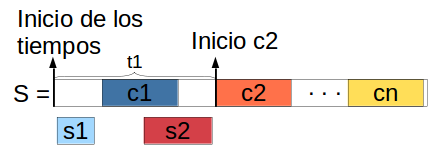
\includegraphics[scale=0.8]{ej2/Graficos/casoA.png}\\
Para que esto pase s1 debe terminar antes de c1, como nuestro algoritmo los coloca según el orden de sus finales esto es absurdo; dado que el algoritmo hubiera colocado primero a s1. \\

\textbf{Caso B:} s2 no se superpone con c1\\
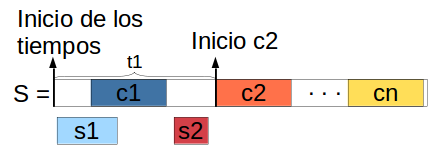
\includegraphics[scale=0.8]{ej2/Graficos/casoB.png}\\
Para que esto pase s2 debe empezar luego del final de c1, y como deben estar dentro del rango, debe terminar antes de c2. Esto es absurdo porque en este caso, al no haber conflicto ni con c1 ni con c2, el algoritmo lo hubiera colocado entremedio de estos.\\
\textit{Observación:} en este caso, el algortimo hubiese elegido s1 en vez de c1 pero esto no modifica la cantidad de cursos de S.\\

El caso en que ambos (s1 y s2) no se superponen con c1 es trivial luego de las explicaciones de los casos A y B.\\
\textit{Observación:} estos casos donde no se superponen prueban que no se puede "sacar"  0 cursos y agregar 1.\\

\newpage
\textbf{Caso C:} ambos (s1 y s2) se superponen con c1\\
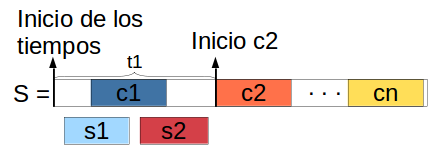
\includegraphics[scale=0.8]{ej2/Graficos/casoC.png}\\
De estas características se desprende que la única forma de que estén dispuestos s1 y s2 es que s1 finalice dentro del rango de c1 y s2 comience dentro del rango de c1.\\
Por lo tanto s1 terminaría antes que c1, es decir, nuestro algoritmo lo hubiese colocado en lugar de c1 y sería el primer curso de la solución. Entonces S no sería la solución dada por el algoritmo.\\

Por lo tanto c1 es una elección correcta y no hay forma de cambiar el curso por otros dos.\\

\textbf{Si se quiere sacar 2 cursos y agregar 3:}\\
Por la explicacion anterios sabemos que c1 está correctamente elegido, entonces la única forma de colocar 3 cursos donde antes había dos es reemplazar c2 por dos cursos. Probandolo de la misma forma que para c1 se llega a un absurdo.\\

Por lo tanto c1 y c2 son elecciones correctas y no hay forma de cambiar dos cursos por otros tres.\\

\textbf{Si se quiere sacar k cursos y agregar k+1:}\\
Extendiendolo de esa forma se llega a que no hay una manera de colocar k+1 cursos.\\

\textit{Nota:} Esto se generaliza para el caso de tomar cursos aleatorios (no sólo adyacentes) ya que la explicación es esencialmente la misma. Elegimos hacerlo en orden sólo por una cuestión de claridad.\\



